% ── Figure 1: Adaptation Trajectory ─────────────────────────────────────────
\begin{figure}[t]
  \centering
  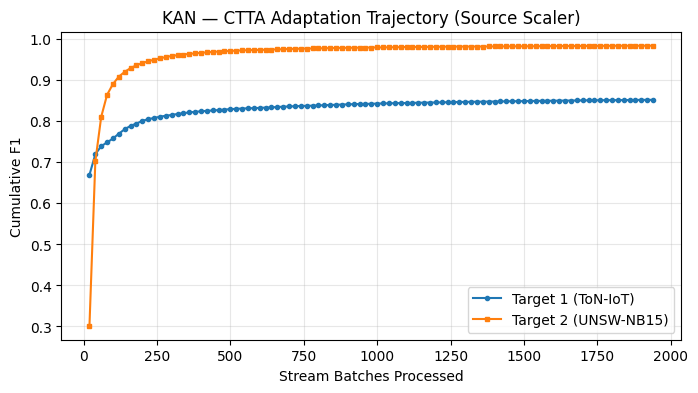
\includegraphics[width=\linewidth]{figures/fig_trajectory}
  \caption{%
    \textbf{Cumulative F1 adaptation trajectory during CTTA}
    (KAN, source: CICIDS2018).
    UNSW-NB15 (orange) reaches ${\approx}1.0$ within the first 50 stream
    batches and plateaus immediately, while ToN-IoT (blue) starts
    higher but converges gradually over ${\sim}2000$ batches.
    The two-speed behaviour reveals that domain proximity governs
    adaptation rate: CICIDS and UNSW share similar benign-traffic
    distributions, enabling near-instant spline recalibration,
    whereas the IoT-centric ToN-IoT shift requires sustained exposure.}
  \label{fig:trajectory}
\end{figure}

% ── Figure 2: Logit Separation ───────────────────────────────────────────────
\begin{figure}[t]
  \centering
  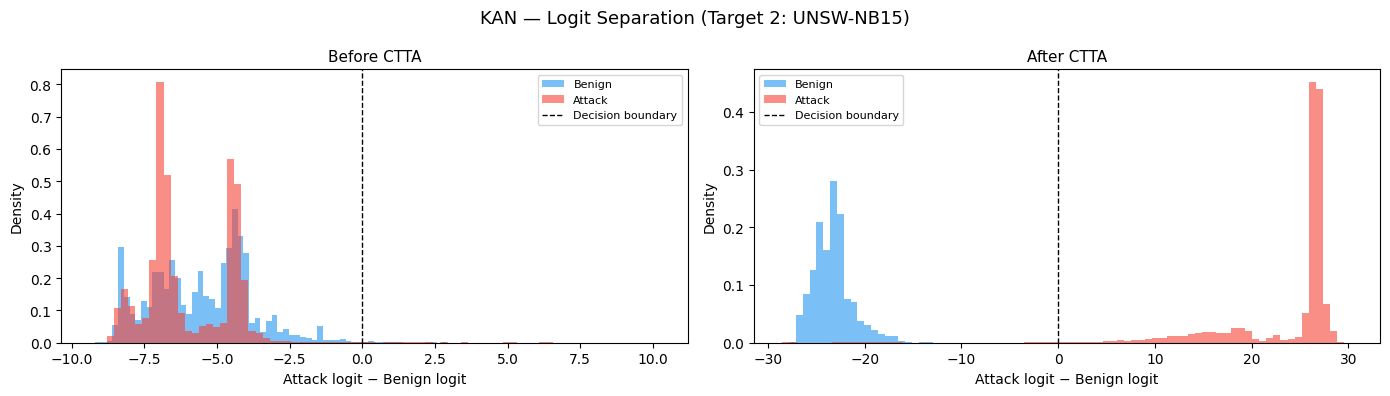
\includegraphics[width=\linewidth]{figures/fig_logit_sep}
  \caption{%
    \textbf{Logit-margin distributions before and after CTTA}
    (KAN, source: CICIDS2018 $\to$ target: UNSW-NB15).
    Before adaptation both class distributions collapse into the same
    narrow $[-10,{+}2]$ band with near-total overlap.
    After spline-only CTTA the benign mass moves to ${\approx}{-25}$
    and the attack mass to ${\approx}{+25}$, with zero overlap,
    corresponding to an F1 jump from $0.007$ to $0.976$.}
  \label{fig:logit_sep}
\end{figure}

% ── Figure 3: Feature Importance Shift (named, full encoder) ─────────────────
\begin{figure}[t]
  \centering
  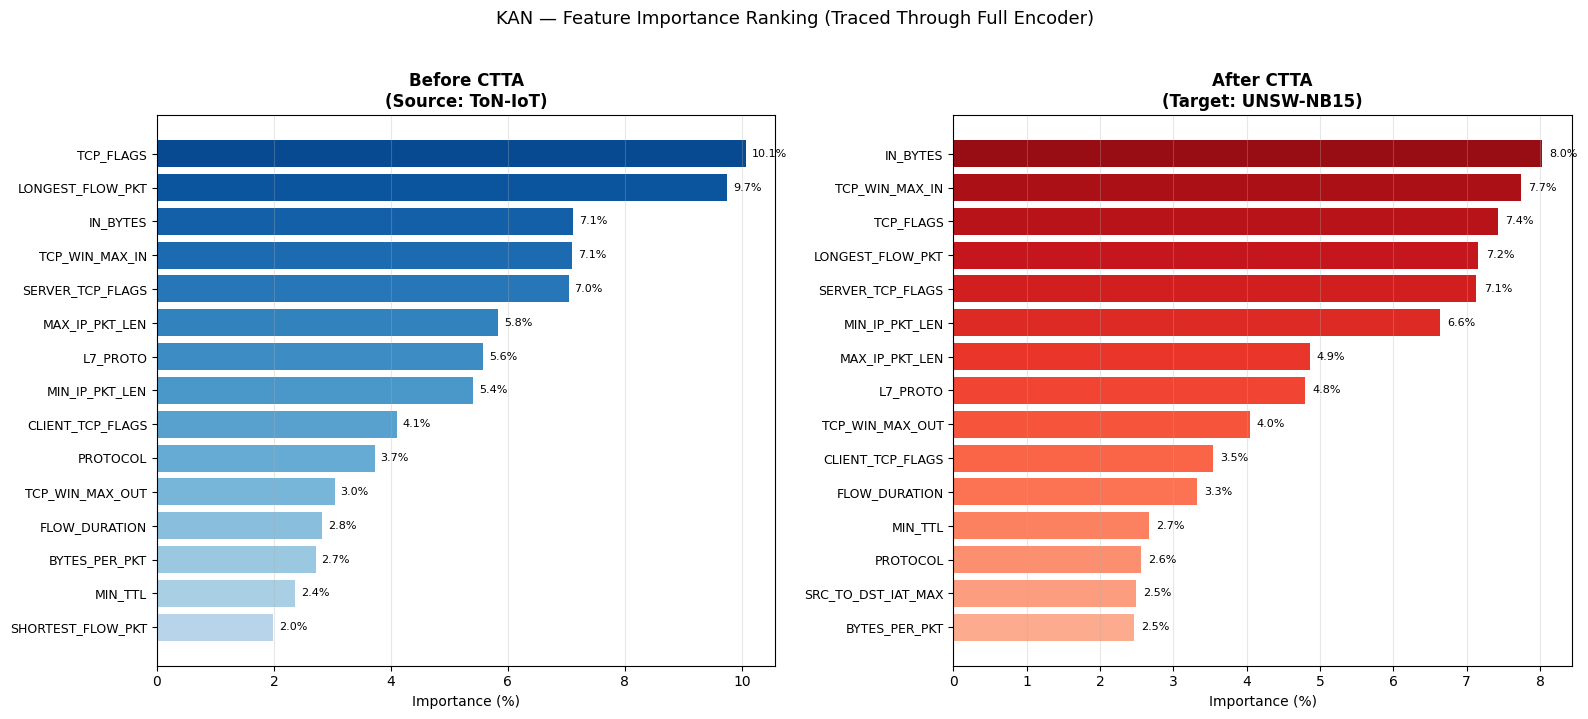
\includegraphics[width=\linewidth]{figures/fig_feat_imp_named}
  \caption{%
    \textbf{End-to-end feature importance before and after CTTA}
    (KAN encoder traced through both layers;
     source: ToN-IoT $\to$ target: UNSW-NB15).
    Importance is computed as $\sum|\mathbf{W}_2|\,|\mathbf{W}_1|$
    and normalised to percentages.
    Adaptation promotes \texttt{IN\_BYTES} from third to first,
    demotes \texttt{TCP\_FLAGS} from first to third, and pushes
    \texttt{LONGEST\_FLOW\_PKT} from second to fourth,
    reflecting the shift from high-rate IoT flows to the
    UNSW-NB15 volume-oriented traffic profile.}
  \label{fig:feat_imp_named}
\end{figure}

% ── Figure 4: Feature Importance Shift (latent layer) ────────────────────────
\begin{figure}[t]
  \centering
  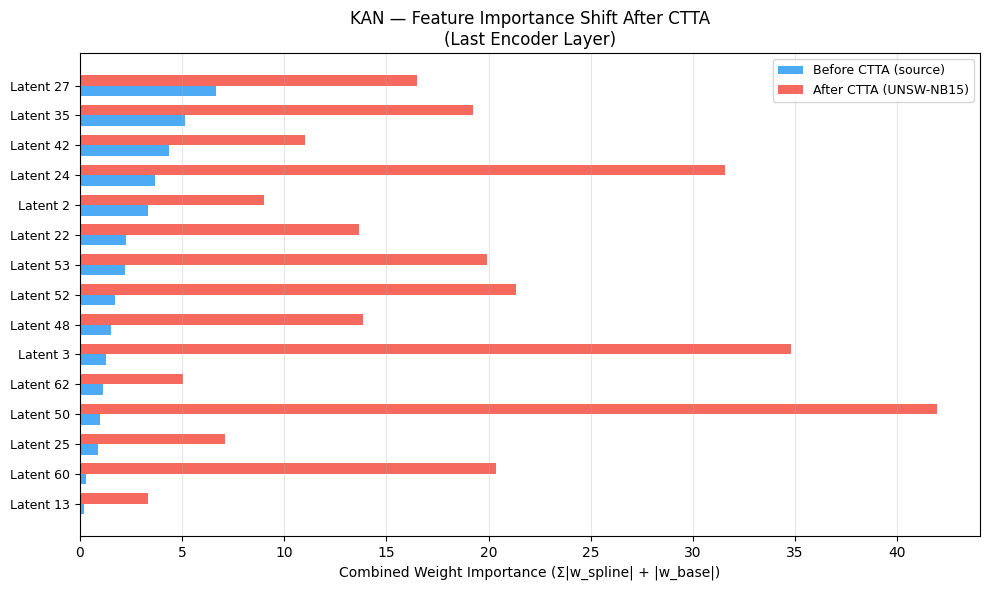
\includegraphics[width=\linewidth]{figures/fig_feat_imp_latent}
  \caption{%
    \textbf{Latent-dimension importance shift in the last encoder layer}
    (KAN, source: ToN-IoT $\to$ target: UNSW-NB15).
    Blue bars show weight magnitudes before CTTA; red bars show the
    same dimensions after spline-only adaptation.
    Dimensions such as Latent~50, 24, and~3 grow by an order of
    magnitude, while the relative ordering changes substantially,
    indicating that the spline coefficients selectively amplify
    target-discriminative latent directions without touching the
    base linear weights.}
  \label{fig:feat_imp_latent}
\end{figure}

% ── Figure 5: KAN Spline Activation Functions ────────────────────────────────
\begin{figure}[t]
  \centering
  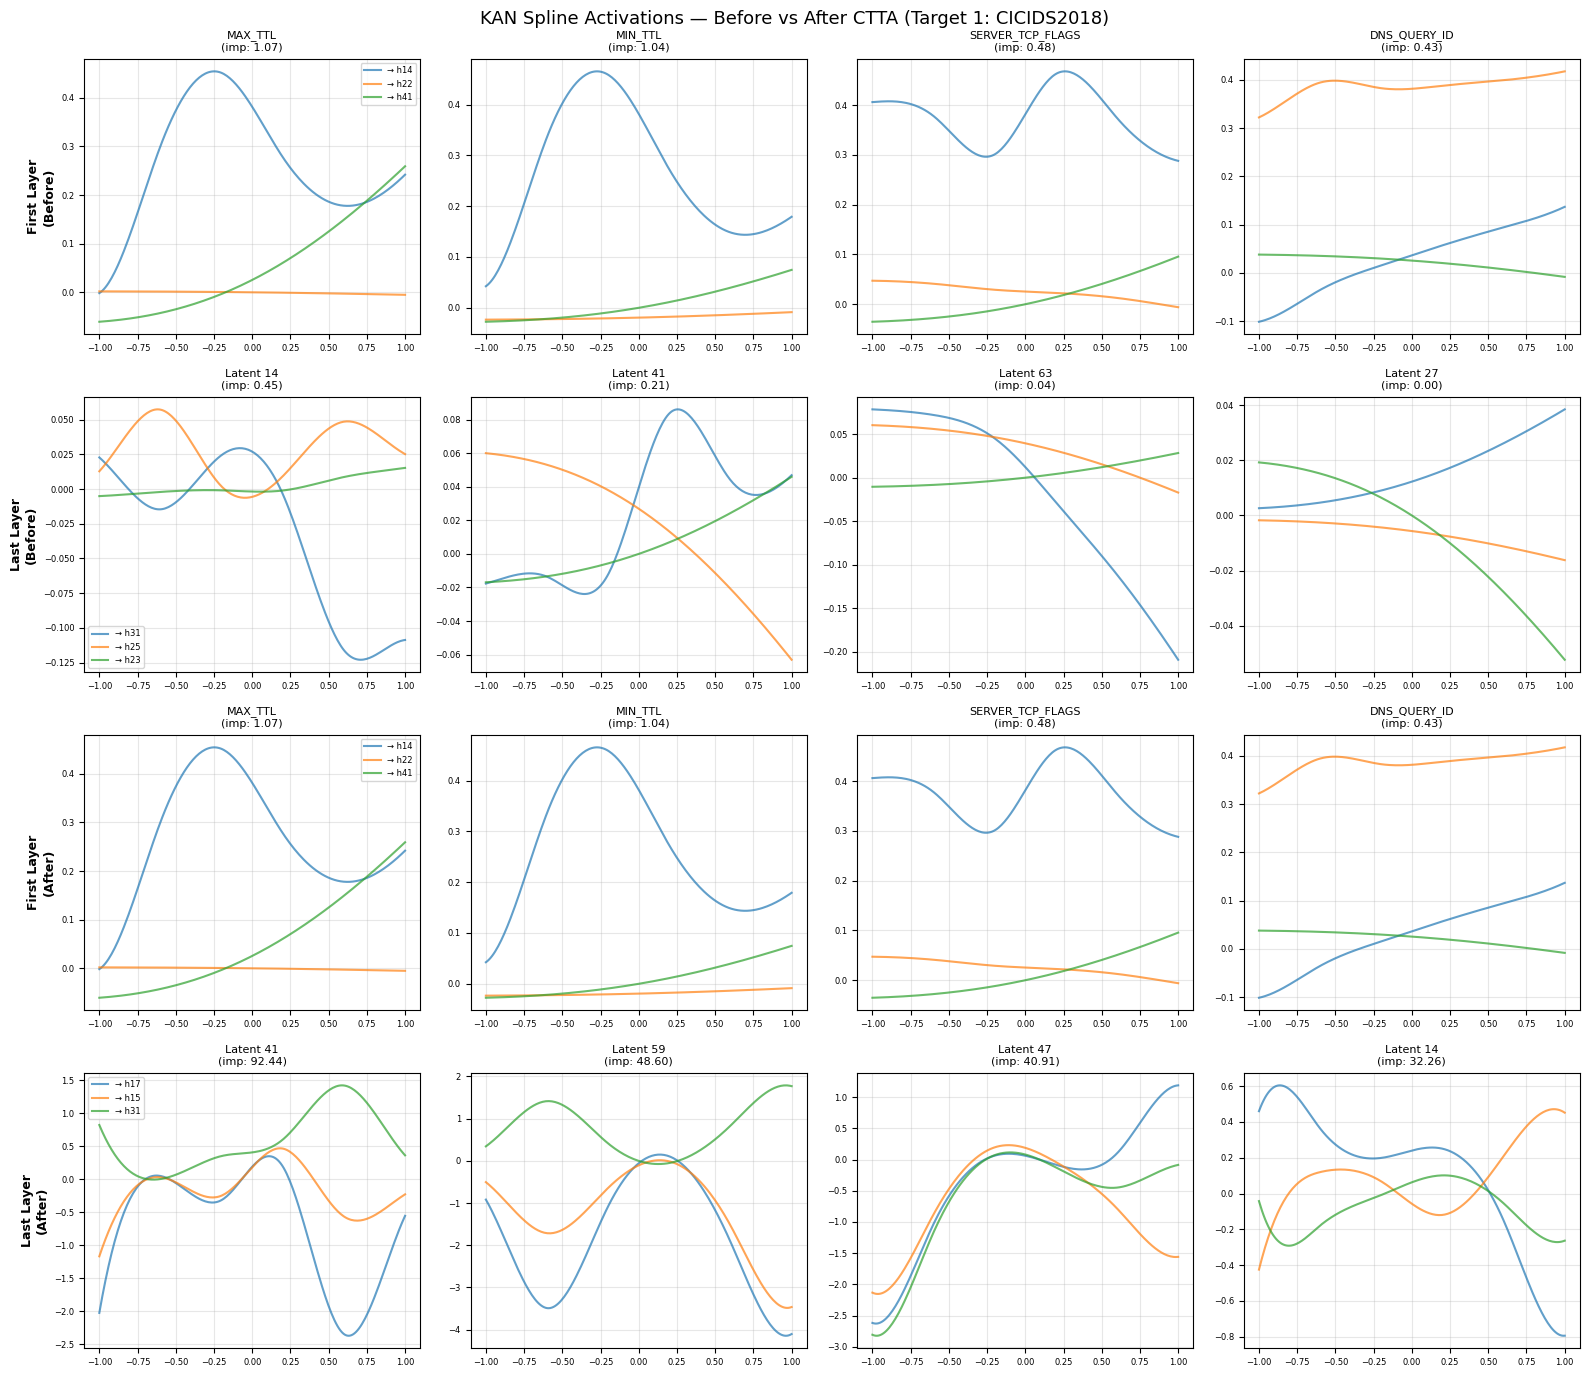
\includegraphics[width=\linewidth]{figures/fig_spline_act}
  \caption{%
    \textbf{KAN spline activation functions before and after CTTA}
    (source: UNSW-NB15 $\to$ target: CICIDS2018).
    Rows~1--2: first and last encoder layer \emph{before} adaptation;
    rows~3--4: the same layers \emph{after} spline-only CTTA.
    Each panel plots the learned univariate mapping for one
    (input feature, hidden neuron) pair.
    Features \texttt{MAX\_TTL}, \texttt{MIN\_TTL}, and
    \texttt{DNS\_QUERY\_ID} exhibit the most pronounced shape changes,
    confirming that effective domain transfer requires reshaping only
    a small, semantically interpretable subset of spline coefficients.}
  \label{fig:spline_act}
\end{figure}
